
\begin{wraptable}{r}{6.5cm} \caption{Summary of SU and disk request for two suites of simulations,
and disk to accommodate our existing archive}
 \label{table1}                                                       
\begin{tabular}{       l               r               r              }
                       &      SU       &    Disk             \\
          \hline                                               
        Galaxies       &5.0\sci{6}       &5.3\sci{3}      Gb     \\
        Turbulence       &3.0\sci{6}       &1.6\sci{3}      Gb     \\
        Analysis       &2.6\sci{5}       &      --             \\
         Archive       &      --       &1.7\sci{5}      Gb     \\
          \hline                                               
                       &8.0\sci{6}       &1.8\sci{5}      Gb       
\end{tabular} \end{wraptable}                                                        
We are requesting \SUrequest\ core-hours on the Anvil supercomputer and \diskrequest\ on the Ranch archival system
in order to perform several simulations.  These simulations are in support of a
campaign to observe gravitational waves from the Big Bang.  


The cosmic microwave background (CMB) contains the oldest light in the universe,
having been emitted 400,000 yr after the Big Bang.  The CMB has been well
studied, and it has taught us many things
about the size, age, expansion, and contents of the Universe.  To learn more, we
must look at its polarization.  The polarization of the CMB contains an imprint
of gravitational waves launched at the Big Bang, which will answer more
questions about the beginning of the Universe.  Unfortunately, the dust and
plasma in the interstellar medium (ISM) of our own Milky Way
Galaxy produces a polarized signal that is much brighter than
the CMB in similar frequencies.  In order to see the primordial polarization, we must first understand
our Galactic polarization.  We will perform simulations in order to understand
the nature of this signal.  In the future we will work to remove it from future CMB experiments such as CMB
S4 and Simons Observatory.  We will perform two suites of simulations; the 
suite of driven \emph{turbulence} will analyze small scale features, and the second is
a suite of full \emph{galaxy} simulations that will cover the large scale and parity
violating signals.

We have been awarded 2\sci{5} SU (Node-hours) on \emph{Frontera} to do two large
scale turbulence simulations and three large scale galaxy simulations.  The
proposed simulations compliment these by covering more parameter space, which is 
necessary for making predictions, at a lower resolution.  Taken together we hope
to make useful predictions about the polarization signature of the interstellar
medium.  

\begin{figure}[t]
\begin{center}
%\includegraphics[width=0.29\textwidth, trim=0cm 0.5cm 0cm 0.5cm, clip]{figs/Fletcher.png}
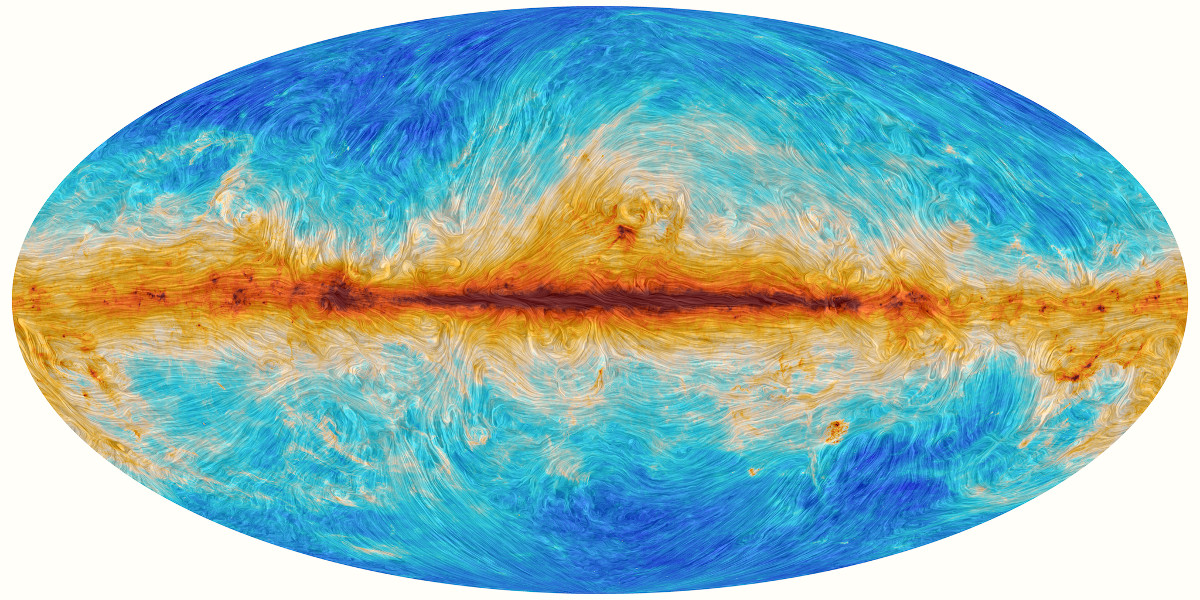
\includegraphics[width=0.65\textwidth, clip]{figs/Planck.jpg}
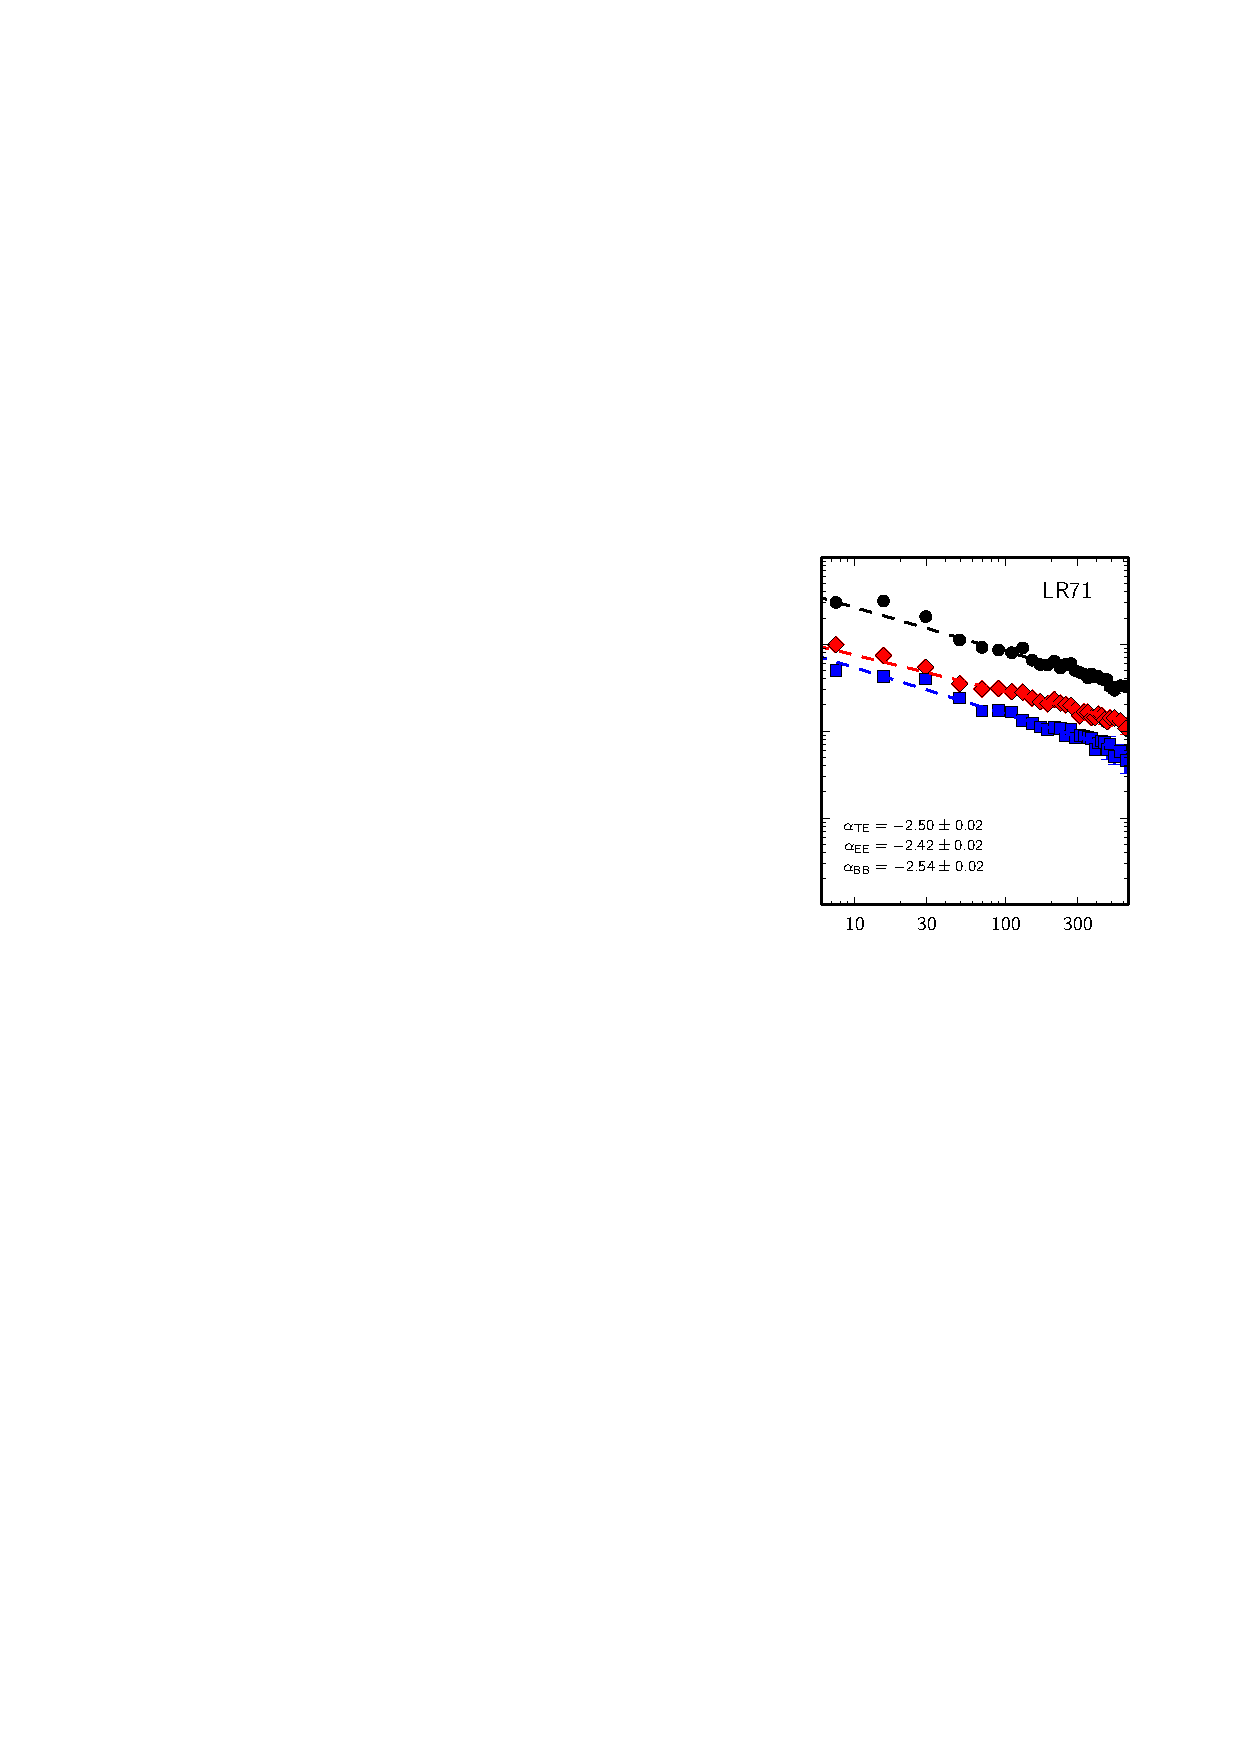
\includegraphics[width=0.27\textwidth, clip]{figs/PlanckForegrounds.pdf}
\end{center}
\vspace{-3mm}
\caption{\label{fig.planck} 
(\emph{Left}) The \emph{Planck} polarization map showing the 353 GHz dust
intensity convolved with the direction of polarization
\citep{PlanckIntermediateXIX15}.  This shows coherent structure on a range of
scales throughout the Milky Way.
(\emph{Right}) The spectrum of polarized emission from the sky, showing
$C_\ell^{TT}$ in
black, $C_\ell^{EE}$ in red, and $C_\ell^{BB}$ in blue.
}
%\vspace{-1mm}
\vspace{-4mm}
\end{figure}



\section{Scientific Background}

The Planck satellite measured the microwave polarization over the whole sky
\citep{Planck18xi}.  Figure
\ref{fig.planck} shows the magnetic field implied by these polarizations (left
panel).  In the ISM, polarization in the microwave is caused by thermal emission
from dust that is lined up along the magnetic field, like iron filings.
Additionally, hot synchrotron electrons also emit in the microwave, and are also
polarized by the magnetic field. These synchrotron electrons occupy  a different part of the galaxy than
the dust due to their higher temperature, and therefore scale height.  

Since polarization is a vector in the plane of the sky, in order to
quantitatively describe it one needs two fields.
Often Stokes parameters, $Q$ and $U$ are used, but these are coordinate
dependent quantities, and $Q$ rotates into $U$ as the telescope rotates.  It is
better to use $E$ and $B$, which are the parity-even and parity-odd combinations
of  $Q$ and $U$.  Roughly, $E$ describes polarization parallel and perpendicular
to filamentary structure that dominates the ISM, and $B$ describes polarization
oblique to filaments.  The spectral signal, of $E$, $B$, and total emission $T$
can be seen in the right panel of Figure \ref{fig.planck}.  It is found that the
emission is distributed as a power law, with spectral slopes of $T$, $E$, and
$B$ all roughly -2.5.  

The correlations between $T$, $E$ and $B$ are also of interest.  The $TB$
correlation was found by Planck \citep{Planck18xi} to be statistically
significant with a correlation coefficient of $r_{TB}=0.05$.  This is
counter-intuitive, as the total emission should be parity even, but $B$ is
parity odd, so the mean should be zero.  This indicates a large scale structure
in the galaxy \citep{Brandenburg20}, 
or some kind of handedness to the filamentary structures in the ISM
\citep{Huffenberger20}.  

In our preliminary work, to appear soon as Stalpes et al (2024, in prep),
we simulated clouds of plasma in the ISM as periodic boxes of supersonically turbulent fluid.
 Simulations of
driven turbulence were performed, wherein kinetic energy is added to the gas at the large
scale, and then cascades to smaller and smaller scales, until the dissipation
scale is reached.  We did this for a range of sonic and \alf\ Mach numbers.  The
sonic Mach number is defined as $\mach=v/c$, where $v$ is the r.m.s velocity and $c$ is the
speed of sound, while the \alf\ Mach number, $\alfmach=v/v_A$, where $v_A$ is
the \alf\ speed, the typical speed for magnetic waves.  Increasing the kinetic
energy of the cloud creates smaller structures, while increasing magnetic field
strength suppresses small structure.  
Our simulations were performed at a modest resolution of
$512^3$.  We found, from synthetic observations of the boxes, that the spectral
slope of $T$, $E$ and $B$ are all reproduced for a (\mach, \alfmach)=(4.7, 1.5).
This is an over simplification, as the true ISM exhibits a range of properties,
but a useful benchmark for future study.
We do not, however, find that the correlations between the three are as large as
those found on the sky.  This implies that there is likely a large scale
structure in the $T$, $E$ and $B$ signals, that comes from the shape of the magnetic field as it is wound around
the galaxy.  

To this end, we are also exploring the polarization signature of full galaxy
simulations that include not only the disk of the galaxy, but the circumgalactic medium
(CGM) that surrounds the galaxy.  By simulating the full galaxy and a large
spatial extent, we will capture the boundary conditions of the nearby (close to
the midplane) magnetic structures as well as the higher latitude structures to
capture the synchrotron signature.  The galactic simulations proposed here aim
to explore the nature of the CGM and its connection to the ISM, as well as the
growth and distribution of the magnetic field around the galaxy.

One of the challenges in understanding the polarization of the CMB foregrounds
is the small spatial scales necessary, as the signal of primordial gravitational
waves lives at the sub-degree scale, as well as the large
scale spatial modes to capture the non-trivial $TB$ correlation, within the general
chaos of a galaxy.  Our multi-tier
approach is essential for covering the range of parameter space the Milky Way
exhibits, and the spatial resolution ultimately necessary to make meaningful
predictions of the foregrounds of the polarized CMB.  The simulations proposed
here (12 simulations of driven turbulence at $1024^3$ and 9 galactic simulations
with a midplane resolution of 12pc) compliment each other in that they capture
both small and large scale features over the range of parameters likely to be
experienced by the ISM.  This also compliments our \emph{Frontera} allocation,
which covers an extremely limited parameter space in exchange for very high
resolution.  The simulations presented here will ensure success of the high
resolution simulations.  In addition, the outstanding memory capacity of
\emph{Anvil} will be a great boon in analyzing the large simulations from the
\emph{Frontera} allocation.  

The ultimate goal is to simulate an entire galaxy with 1 pc resolution.  Our
proposed galaxy simulations are an AMR stack with approximately $256^3$ zones
per level for 8 levels, with an outer box size of 8192pc and a finest resolution
of 12.5 pc.  The \emph{Frontera} simulations double the resolution at every
level and achieve 6.25pc resolution.  Once we are successful with these
simulations, we will extend to $1024^3$ per level for 8 levels, which will get
3.125pc resolution at the midplane of the galaxy.  We will ultimately
combine the knowledge gained from our $2048^3$ simulations,  the simulations of our $512^3$
tower, and the experience and preliminary science gained in the currently
proposed simulations to launch simulations of galaxies at 1pc resolution at the
midplane.

We describe the code to be used in Section \ref{sec.methods}. A detailed
description of the  simulations  to be performed is in Section
\ref{sec.simulations}, and the detailed accounting of the disk and SU request is
in Section \ref{sec.request}. The interaction with the other allocation in
Section \ref{sec.others}.


